\documentclass[tikz,border=10pt]{standalone}
\usepackage{amsmath}
\usetikzlibrary{arrows.meta}

\begin{document}

{\sffamily\everymath{\sf}

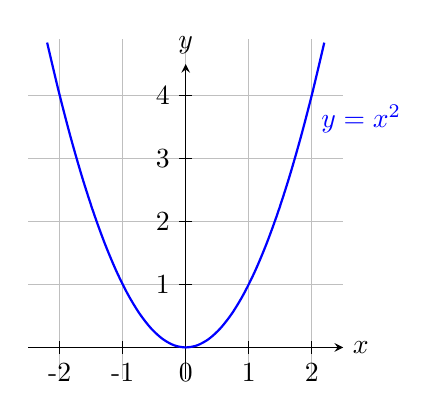
\begin{tikzpicture}[scale=0.8, >=stealth]

  % Faint grid
  \draw[very thin, color=gray!50] (-2.5,-0.5) grid (2.5,4.9);

  % Axes
  \draw[->] (-2.5, 0) -- (2.5, 0) node[right] {$x$};
  \draw[->] (0, -0.5) -- (0, 4.5) node[above] {$y$};

  % Tick marks and labels
  \foreach \x in {-2,...,2}
    \draw (\x,0.1) -- (\x,-0.1) node[below] {\x};
  \foreach \y in {1,...,4}
    \draw (0.1,\y) -- (-0.1,\y) node[left] {\y};

  % Parabola y = x^2 in blue
  \draw[domain=-2.2:2.2, smooth, variable=\x, blue, thick]
    plot ({\x}, {\x*\x});

  % Label
  \node[blue, below right] at (2,4) {$y = x^2$};

\end{tikzpicture}

}

\end{document}
